\subsection{Preprocessing techniques}
%In this section, we consider the attack information as noise in the image. We assume attackers tend to control the magnitude of their attacks so as not to be detected by the system, but make them effective enough to misguide the system to the wrong results. We then make use of this effect, and consider the problem from the image preprocessing perspective. We use different approaches, rescaling, bit-depth reduction, total variation and , to remove the attack or adversarial perturbations in the input data before we fit into the net, and also try to maintain enough information for our net to give the right results.

In this section we consider a grey-box setting where the attacker knows the structure of the neural network for the image classifier, however during testing, we impose further transforms on test samples. This is designed to obscure the gradients so that adversarial perturbation effects can be reduced. We looked at a range of preprocessing techniques based on \cite{Guo18}: image resolution reduction, bit-depth reduction, total variation denoising and randomised crop-and-rescale.


\subsubsection{Bit-Depth Reduction} %reference needed here
The bit-depth reduction approach \cite{DBLP:journals/corr/XuEQ17} aims at reduciing the colour depth in bits, in order to remove the adversarial attack but to not significantly destroy the recognisability of the images at the same time. 

Our input values are in the range [0,1]. We then apply the approach to reducing the image from 8 bits to i bits by, first multiplying the input data by ($2^i - 1$), then rounding to integers, and finally scaling the values back to the the range [0,1].

\begin{figure}[h!]
	\centering
	\begin{subfigure}{.35\textwidth}
		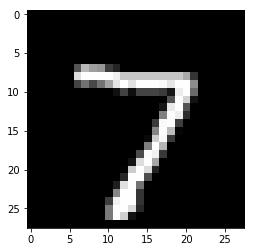
\includegraphics[width=\textwidth]{original7.png}
		\caption{Original image}
		\label{fig: bit-depth reduction 1}
	\end{subfigure}
	\begin{subfigure}{.35\textwidth}
		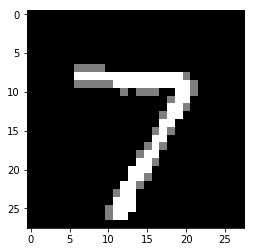
\includegraphics[width=\textwidth]{bit1-7.png}
		\caption{bit-two image}
		\label{fig: bit-depth reduction 8}
	\end{subfigure}
	\caption{Bit-depth reduction image}
\end{figure}

We can see for MNIST database, even we reduce the color depth to two bits, it is very clear and does not introduce human-observable loss, which also encourages us apply it to defend our system. 


\subsubsection{Median, LAP and LAR Smoothing Filters}
It has been shown that by implementing median filtering, local average with neighbourhood pixels (LAP) and the local average with radius (LAR) pre-processing noise filters on the input image data it is possible to effectively reverse the mis-classifications caused by adversarial perturbations and significantly decrease the efficiency of the attack \cite{khalid2019fademl}. 

\begin{figure}[h!]
	\centering
		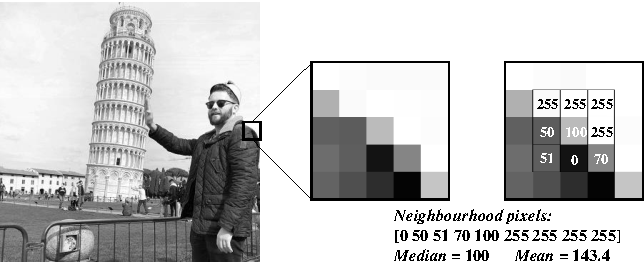
\includegraphics[width=.72\textwidth]{Diagram1-cropped.pdf}
		\caption{Original image}
		\label{fig: Median}
	\caption{Median filtering to remove impulse (or salt-and-pepper) noise}
\end{figure}
These standard noise filtering algorithms are easy to implement and can significantly retrieve correct classification confidence lost to the perturbations, whilst maintaining the visual structure of the image. Other forms of pre-processing methods which are also feature-preservative include JPEG compression (lossy image compression) where the image is irreversibly encoded so as to reduce the file size, and image quilting where a novel image is created by merging together smaller patches of images which already exist \cite{efros2001image}.


\begin{figure}[h!]
	\centering
	\begin{subfigure}{.3\textwidth}
		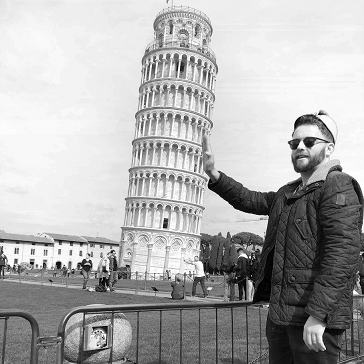
\includegraphics[width=\textwidth]{Iorig.png}
		\caption{Original image}
		\label{fig: LAPLAR1}
	\end{subfigure}
	\begin{subfigure}{.3\textwidth}
		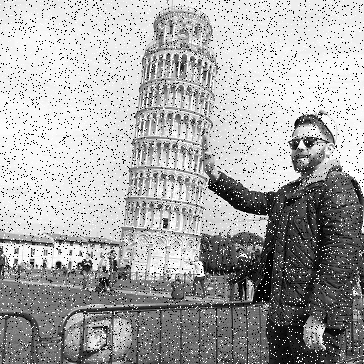
\includegraphics[width=\textwidth]{Inoise.png}
		\caption{Impulse noise inserted}
		\label{fig: LAPLAR2}
	\end{subfigure}
	\begin{subfigure}{.3\textwidth}
		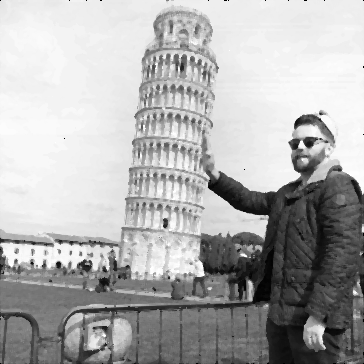
\includegraphics[width=\textwidth]{Ifiltered.png}
		\caption{Median filtering noise}
		\label{fig: LAPLAR3}
	\end{subfigure}
	\caption{Median filtering to remove impulse (or salt-and-pepper) noise}
\end{figure}
Despite the promising experimental results these pre-processing filters have shown \cite{khalid2019fademl}, the percentage confidence allocated to a given classification is still eroded (albeit much less). Based on their own results, the same authors also developed a novel noise-Filter-aware Adversarial ML ($FAdeML$) attack which was able to trick a network into mis-classifying image data even after the application of these pre-processing algorithms. Clearly this research requires more work to quantify the effectiveness of pre-processing noise filters on combatting adversarial attacks (especially with the development of adversarial attacks which take noise filters into consideration), however it seems irrefutable that the benefits of using these filters far outweighs any minor degradation in image quality due to the filtering.



\subsubsection{Total Variation Minimisation} 
Another preprocessing approach we consider is a compressed sensing approach that drop pixels via total variation minimisation \cite{Rudin:1992:NTV:142273.142312}. This method selects a small portion of pixels randomly, and then replace it by minimising the variation from pixels nearby. Strictly speaking, we first select pixels by sampling a Bernoulli random variable $X(i,j,k)$ for pixel at the location $(i,j,k)$, set the value $p$ to control the amount of pixels chosen to change, and maintain the pixel if $X(i,j,k) = 1$. Then we replace the values in the chosen pixels by minimising the variation of the whole input image, the so called total variation, 
\begin{align}
	\min_{\mathbf{z}}||(1 - X) \odot (\mathbf{z} - \mathbf{x})||_2 + \lambda_{TV}\cdot TV_p{\mathbf{z}}.
	\label{equ: tv obj}
\end{align}
Here $\odot$ denotes element-wise multiplication, and $TV_p{\mathbf{z}}$ represents the $L_p$-total variation of $\mathbf{z}$:

\begin{align}
	TV_p{\mathbf{z}} = \sum_{k = 1}^{K}\left[\sum_{i=2}^{N}||z(i,:,k) - z(i-1, :, k)||_p + \sum_{j = 2}^{N}||z(:,j,k) - z(:,k-1,k)||_p\right].
\end{align}

The total variation measures the amount of variation both column-wise and row-wise in the image $\mathbf{z}$, and the minimisation of it encourages the removal of small perturbations in the image, which coincides with the features we assume of adversarial perturbations. The objective function \ref{equ: tv obj} is convex in $\mathbf{z}$, hence we can solve for it efficiently, and in the following implementation we choose $p = 2$ and utilise a solver proposed by Chambolle \cite{Chambolle:2004:ATV:964969.964985}. 


\subsubsection{Defence GAN}
In considering solutions to the pre-processing defence to adversarial attacks, in particular FGSM, we note that all our proposed methods are attempting in some way to smooth out the noise in a poisoned image and classify the result. An alternative is to ask can we classify a different image with the same semantic content as the poisoned image but without the poison.  This method suggests we could use a generative model of our dataset to generate in domain data which would remove any chance of classifying a poisoned image.  The remaining question is how to condition the generator to create images with the same semantic content of the poisoned image without introducing the poison to our approach?

This idea has been recently introduced by [TODO citation] where they report good success in defending againsts adversarial attacks.


\subsubsection{Image Resolution Reduction}
Most of the time, humans can make out numbers and objects from very low resolution images, this suggests that the defining features of classes are fairly general going from image to image. Therefore intuitively, we expect that if we decrease the resolution by scaling the image to a smaller size then rescaling back, using for example a bilinear interpolation, then the transformed image should still be recognisable (given that the scaling is not too extreme). Since this means there is a local pooling of information, it will be interesting to see if adding such a transformation to all test samples will be more robust against perturbation based attacks.

\subsubsection{Randomised crop and rescaling}
One way of obscuring the gradient of the neural network is to add some random operations during the testing. Randomised crop and rescaling involves taking a random crop of the original image and then rescale back to the desired size. Note that typically a range or proportion is specified so that the image post-cropping can still be recognisable as the original object. 

The neural network is trained on the original images, but when it comes to testing, all test samples are subjected to random transform as described above. Often we take multiple random crop-and-rescaling of the same test image and feed all such transformed images into the neural network. We can then find some summary statistic from all the transformation to classify this image. For example, we can take the mode of the classification or find the maximum of the average sigmoid output value in the final layer of the neural network. 

Of course this means that there are additional computation cost added to the testing phase. However since this is obscured to the attacker, an FGSM attack should be less effective. We also expect that increasing the number of transformed images on a test image should also increase accuracy.

